\documentclass[10pt]{article}
\usepackage[]{mcode}
\usepackage{graphicx}
\usepackage[font=small,labelfont=bf]{caption}

\begin{document}
\section{Central Limit Theorem}
Consider a sample of 1000 observations from a Uniform or Gaussian population distribution. These distributions have been recorded and binned into histograms in figure 1 and 2 below. As expected the uniform distribution follows a roughly box shaped probability density function and the Gaussian distribution follows the well known 'Bell shaped curve'. 

%\\ \mcode{distHist(1000, 'uniform'); distHist(1000, 'gaussian');}
%\lstinputlisting{C:/Users/Alun/Documents/Work/DataScience/Southampton/Machine_learning/MachineLearning/Labone/distHist.m}

\begin{figure}[!h]
  \centering
  \begin{minipage}[b]{0.4\textwidth}
    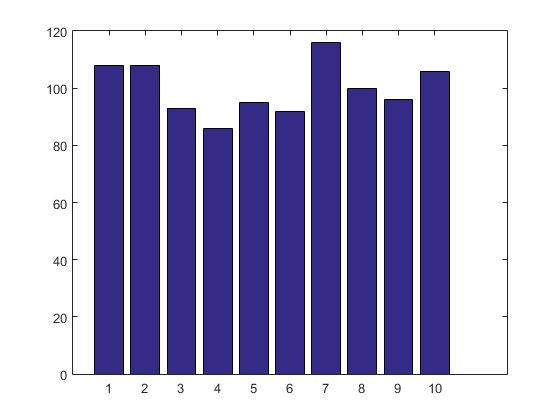
\includegraphics[width=\textwidth]{uniform.jpg}
    \caption{Sampling Uniform Distribution}
  \end{minipage}
  \hfill
  \begin{minipage}[b]{0.4\textwidth}
    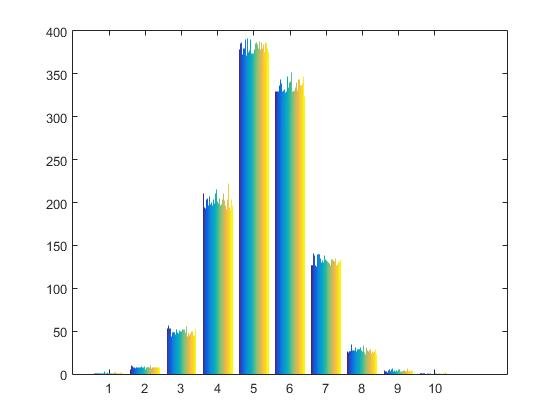
\includegraphics[width=\textwidth]{gaussian.jpg}
    \caption{Sampling Normal Distribution}
  \end{minipage}
\end{figure}

%\lstinputlisting{C:/Users/Alun/Documents/Work/DataScience/Southampton/Machine_learning/MachineLearning/Labone/clt.m}

The central limit theorem states that if we take a sample of a population distribution and apply a statistic to it, for instance calculate the mean or sum of the sample then the distribution of our statistic itself approximates a Normal distribution, centred on the mean of the population distribution and with variance of $s^2 = \frac{\sigma^2}{n}$. This principal is true regardless of the population distribution originally sampled, for example in figures 3,4,5 below a uniform distribution has been sampled to produce a statistic. 

The approximation limits to the Gaussian distribution for large samples of n, although different population distributions can limit at different rates. Shown below are histograms sampling the difference between Two 12 observation samples of a uniform distribution for different sample sizes. 

\begin{figure}[!h]
  \centering
  \begin{minipage}[b]{0.32\textwidth}
    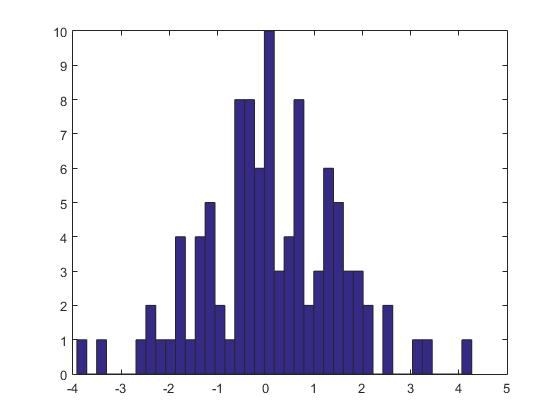
\includegraphics[width=\textwidth]{clt100.jpg}
    \caption{10 Samples}
  \end{minipage}
  \hfill
  \begin{minipage}[b]{0.32\textwidth}
    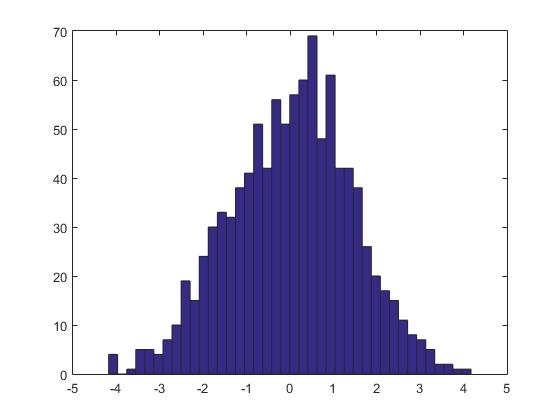
\includegraphics[width=\textwidth]{clt1000.jpg}
    \caption{1000 Samples}
  \end{minipage}
  \begin{minipage}[b]{0.32\textwidth}
    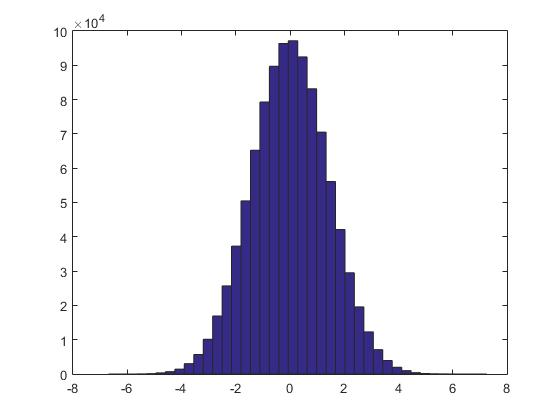
\includegraphics[width=\textwidth]{clt100000.jpg}
    \caption{100000 Samples}
  \end{minipage}
\end{figure}

We can see the distribution approximates to a bell shaped curve for large values of n. Also The variance of the distribution decreases for larger values of n, with data typically sitting closer to the mean. 

\section{}
\subsection{Manipulating covariance}

Multi-dimensional normally distributed datasets can be produced with desired shapes as long as the desired covariance matrix is known. To produce these distributions first factorise the desired covariance matrix to produce the matrix A such that $A'A = C$. Then compute the product of our two dimensional normal distribution X and A $Y = X*A$. This has been done for an example covariance matrix C = [2,1; 1,2] in figure 6 below. 

\begin{figure}[!h]
  \centering
  \begin{minipage}[b]{0.3\textwidth}
      \includegraphics[width=\textwidth]{twoDGaussian.jpg}
      \caption{Normal distribution (teal) \& manipulated distribution (pink)}
  \end{minipage}
  \hfill
  \begin{minipage}[b]{0.3\textwidth}
     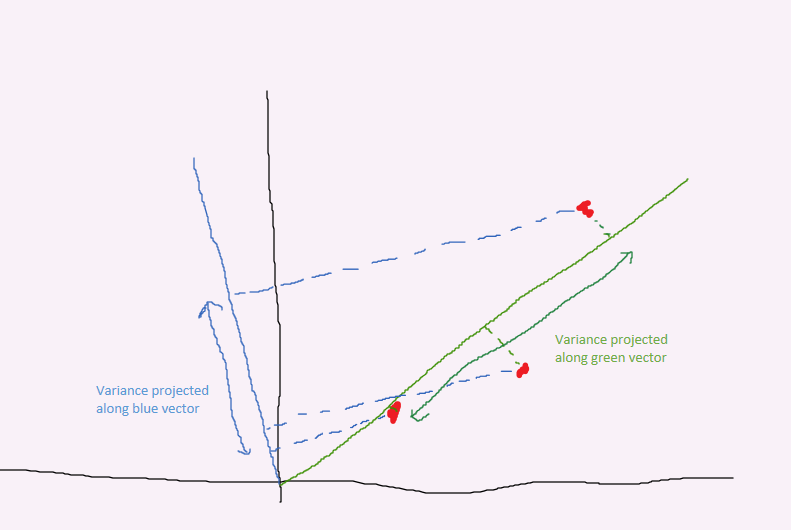
\includegraphics[width=\textwidth]{varianceProjection.png}
     \caption{Doodle describing how dot product projects the variance}
  \end{minipage}
  \begin{minipage}[b]{0.3\textwidth}
     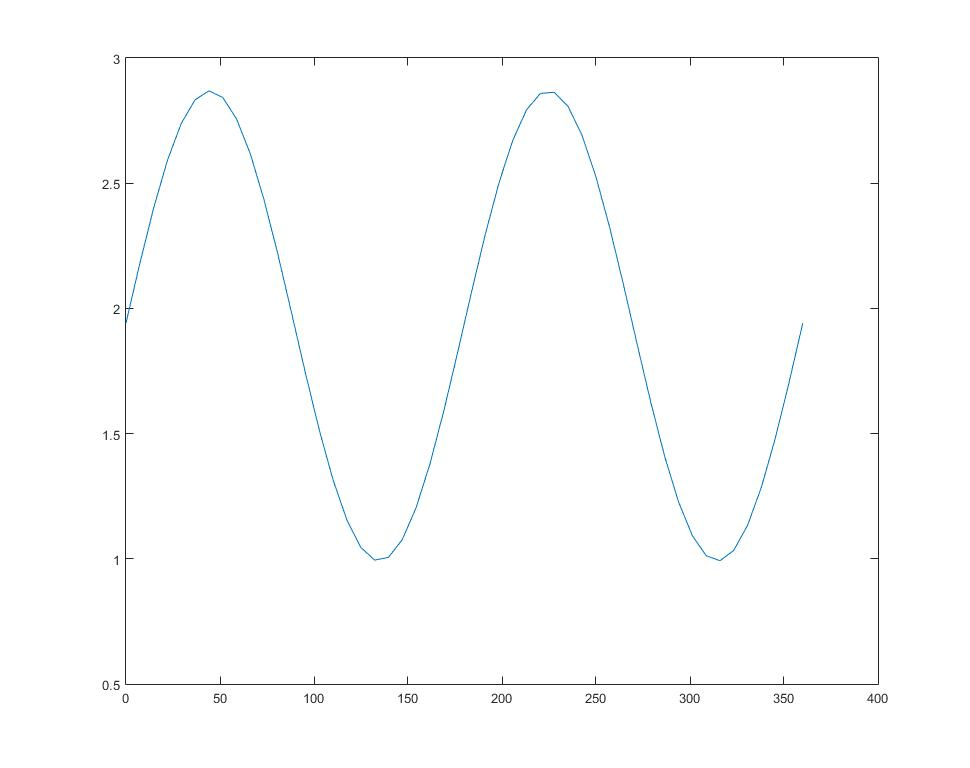
\includegraphics[width=\textwidth]{variance.jpg}
     \caption{How projected variance varies with angle (degrees)}
  \end{minipage}
\end{figure}

Using the cov() function in matlab yields a covariance of C verifying our goal of producing a desired covariance.

\subsection{Dimensionality reduction}  
In dimensionality reduction the desire is to simplify the features of a dataset while retaining as much information as possible. This is done by projecting the n dimensional data onto a lower dimension plane, for example a vector. In order to choose the vector to project onto, we want to minimise the information lost. Intuitively we can do this by trying to maximise the variance of our data along the vector (once projected each observation is described only by its position on the vector, so variance of this position is an analogue to data retention). Figure 7 shows the mechanism for this. $ X*u $

The vector $u = [sin(theta_); cos(theta)]$ for $\theta \in {0-2\pi}$ draws a circle from the origin. As the projection vector rotates in a circle we can see how well fitted the different lines are to our data. We can see from the plot that the projection which has maximum variance (closest to the natural projection of the data) is slightly below 50 degrees. By maximising the variance of the projection we can maximise the information retained from the dimensionality reduction process. 

Using matlab's $eig()$ function we can extract the eigenvectors of the covariance matrix. The first eigenvector is equal to the principle component, the second is orthogonal to this. We can see that the eigenvectors of a covariance matrix describe this vector of maximum variance (priciple component). If the covariance matrix is symmetric this result can be generalised INSERT REFERENCE.


\end{document}

